
In this section, we present a Lagrangian-based model capable of describing the dispersed phase with an arbitrary order of accuracy.

\subsection{Fundamental properties}

At this stage, we define some fundamental properties associated to each particle labelled $\alpha$.
Following the strategy of \citet{lhuillier2009rheology,lhuillier1992volume,zaepffel2011modelisation} and \citet[Chapter 2]{morel2015mathematical}
we define the mass $m_\alpha$, position of center of mass $\mathbf{x}_\alpha$, momentum $\textbf{p}_\alpha$ and total energy $E_\alpha^\text{tot}$, of the particle $\alpha$, as
\begin{align}
    m_\alpha(t)
    = \intO{ \rho_2  }, 
    &&
    \textbf{x}_\alpha(t)
    = \frac{1}{m_\alpha(t) }\intO{ \rho_2 \textbf{x} }, 
    \label{eq:mass_pos}
    \\
    \textbf{p}_\alpha(t) 
    = \intO{ \rho_2 \textbf{u}_2^0 }.
    &&
     E_\alpha^\text{tot}(t) 
    = \intO{ \rho_2 [e_2^0 + (u_2^0)^2/2] },
    + \intS{ \gamma },
    \label{eq:momentum_energy}
\end{align}
 $\Omega_\alpha(t)$ is the time-dependent domain occupied by the particle $\alpha$ (see \ref{fig:Scheme}). 
Note that the total energy of the particle is the integral of the local total energy $\rho_2 [e_2^0 + (u_2^0)^2/2]$ over its volume and the integral of the local surface energy, $\gamma$ over its surface. 
Additionally, in the following we note $s_\alpha = \intS{}$ the surface of the particle $\alpha$. 
Subsequently, we define the velocity of the particle center of mass, denoted as $\textbf{u}_\alpha$ by 
\begin{equation}
\textbf{u}_\alpha = \frac{d \textbf{x}_\alpha}{dt}  
\end{equation}
Replacing $\textbf{x}_\alpha$ by its definition (\ref{eq:mass_pos}) we obtain
\begin{equation}
    \textbf{u}_\alpha = \frac{1}{m_\alpha}
    \frac{d}{dt} 
    \left(
        \intO{ \rho_2 \textbf{x} }
    \right)
    - \frac{1}{m_\alpha^2} \frac{d}{dt} \left(\intO{ \rho_2 } \right)
    \intO{ \rho_2 \textbf{x} }.
\end{equation}
%\tb{ A finaliser
Using the Reynolds transport theorem (\ref{eq:reynolds_transport}) for both term in parenthesis and making use of the conservation of mass (\ref{eq:dt_rho}) and the definition of $\textbf{x}_\alpha(t)$ (\ref{eq:mass_pos}) in the last term, gives
\begin{equation}
    \textbf{u}_\alpha = 
    \frac{1}{m_\alpha}\intO{ \left[
        \pddt (\rho_2 \textbf{x}) + \div\left(\rho_2 \textbf{x}\textbf{u}_2\right) 
    \right]} \\
    + \frac{1}{m_\alpha}\intS{ \textbf{x} \rho_2(\textbf{u}_I   - \textbf{u}_2) \cdot \textbf{n}_2 }
    -  \frac{\textbf{x}_\alpha}{m_\alpha}    \intS{ \rho_2(\textbf{u}_I   - \textbf{u}_2) \cdot \textbf{n}_2 }
\end{equation}
Then by considering the mass conservation for the first term, noticing that $\grad \textbf{y} = \bm\delta$ where $\bm\delta$ is the identity tensor for the second term, and introducing $\mathbf{r} = \mathbf{y} - \mathbf{y}_\alpha$ for the last two terms gives, 
\begin{equation}
    \textbf{u}_\alpha(t) = \frac{1}{m_\alpha(t)} \left(
        \textbf{p}_\alpha(t)
        +  \int_{\Gamma_\alpha(t)} \rho_2 \textbf{r} (\textbf{u}_I^0 - \textbf{u}_2^0)\cdot \textbf{n}_2 d\Sigma
        \right),
        \label{eq:dt_y_alpha}
\end{equation}
where $\textbf{r}(\textbf{x},t) = \textbf{x} - \textbf{x}_\alpha(t)$. 
In \ref{eq:dt_y_alpha}, it can be observed that the first component of the velocity represents the linear momentum divided by the mass of the particle. 
This corresponds to the mass-averaged velocity over the volume of the particle.
The second term in \ref{eq:dt_y_alpha} arises from the contribution of anisotropic mass transfer across the surface of the particle. 
This mass transfer leads to the motion of the particle's center of mass, thereby contributing to the total velocity.
To illustrate this concept, let us consider a fixed drop with no momentum lying over a very hot plate.
In this scenario, we assume that the plate is sufficiently hot to induce evaporation, specifically on the bottom portion of the drop.
Hence, under the effect of an anisotropic evaporation flux one may expect the second term to be non-negligible.
Consequently, the center of mass of the drop has a non-zero velocity in the opposite direction of the plate, even though the momentum is assumed to be zero.
Note that \ref{eq:dt_y_alpha} generalized usual expression of the center of mass velocity whom neglect the second term.
In the following, for the sake of brevity we discard the time dependency notation for all Lagrangian quantities denoted by the subscript $_\alpha$ and in particular $\Gamma_\alpha$ and $\Omega_\alpha$.
Nevertheless, the reader must understand that all Lagrangian quantities and integration domains subscribed by $_\alpha$ are time dependent. 

The particle's internal relative motions or the \textit{inner velocity} is given by $\textbf{w}_2^0(\textbf{x},t) = \textbf{u}_2^0(\textbf{x},t) - \textbf{u}_\alpha(t)$. Then the momentum of the particle reads
\begin{equation}
    \label{eq:momentum_definition_1}
    \textbf{p}_\alpha
    = m_\alpha \textbf{u}_\alpha
    + \int_{\Omega_\alpha} \rho_2 \textbf{w}_2^0 d\Omega.
\end{equation}
Alternatively, from \eqref{eq:dt_y_alpha}, we obtain,
\begin{equation}
    \textbf{p}_\alpha
    =  m_\alpha \textbf{u}_\alpha
    - \int_{\Gamma_\alpha} \rho_2\textbf{r}(\textbf{u}_I^0 - \textbf{u}_2^0)\cdot \textbf{n}_2 d\Sigma
    \label{eq:momentum_definition}
\end{equation}
Therefore, the momentum of a particle can be seen as a sum of the mean velocity plus the integral of the fluctuation (\ref{eq:momentum_definition_1}), with the latter being equivalent to minus the first moment of mass transfer term (\ref{eq:momentum_definition}).
Indeed, by identification we obtain : $\intO{ \rho_2 \textbf{w}_2^0 } = - \intS{  \rho_2\textbf{r} (\textbf{u}_I^0 - \textbf{u}_2^0)\cdot \textbf{n}_2 }$. 
%The essential aspect of this relation highlighted here is that 
Hence the internal velocity fluctuations within a fluid particle do not contribute to the total linear momentum $\textbf{p}_\alpha$, as long as the anisotropic mass transfer is negligible.  

Carrying similar procedures, the total energy $E_\alpha^\text{tot}$ can be decomposed according to,
\begin{equation*}
    \label{eq:E_alpha_def}
    E_\alpha^\text{tot}
    = m_\alpha e_\alpha 
    + W_\alpha
    + m_\alpha (u_\alpha)^2/2
    + \gamma s_\alpha 
    + \textbf{u}_\alpha \cdot  \intS{  \rho_2 \textbf{w}_2^0 }
    + \intS{  \rho_2 \textbf{w}_2^0 } \cdot \textbf{u}_\alpha 
\end{equation*}
Consequently, the total energy of a particle is the contribution of :
its internal energy $m_\alpha e_\alpha$; 
its internal kinetic energy, $W_\alpha = \int_{\Omega_\alpha(t)} \rho_2  (w_2^0)^2/2 d\Omega$;
its center of mass kinetic energy, $u_\alpha^2/2$; 
its surface energy $\intS{ \gamma} = \gamma s_\alpha$; 
And finally two mass transfer related terms $\textbf{u}_\alpha \cdot  \intS{  \rho_2 \textbf{w}_2^0 }$ and $\intS{  \rho_2 \textbf{w}_2^0 } \cdot \textbf{u}_\alpha$. 

\subsection{Conservation laws}

We assign to a particle indexed, $\alpha$, occupying the domain $\Omega_\alpha$ (see \ref{fig:Scheme}) an arbitrary Lagrangian property $q_\alpha$ defined by $q_\alpha  = \intO{ f_2^0}$.
Similarly, we define $q_{I\alpha} = \intS{ f_I^0}$ as being an integrated surface property .
\subsubsection{Inside the volume }
To describe the evolution of any arbitrary Lagrangian quantity $q_\alpha$, we need to establish its time derivative.
Since, $q_\alpha$ is an integral quantity with a time-dependent domain of integration, we apply the general Reynolds transport theorem for volume integral which gives for material domain (the droplet volume),
\begin{equation}
    \ddt  \intO{f_2^0}
    = \intO{\left[ \pddt f_2^0 + \div\left(f_2^0\textbf{u}_2^0\right) \right]}\\
    + \intS{ f_2^0 (\textbf{u}_I^0-\textbf{u}_2^0)\cdot \textbf{n}_2 }.
    \label{eq:reynolds_transport}
\end{equation}
By substituting the integrand of the first integral on the right-hand side (RHS) with \ref{eq:dt_f_k} and making use of the divergence theorem we obtain the conservation laws of the quantity $q_\alpha$, namely,  
\begin{equation}
    \ddt{q_\alpha}
    = \intO{ s_2^0 }
    + \intS{ \left[
        f_2^0 (\textbf{u}_I^0-\textbf{u}_2^0) 
        + \mathbf{\Phi}_2^0 
        \right] \cdot \textbf{n}_2 },
    \label{eq:dt_q_alpha}
\end{equation}
where we have use the Gauss divergence theorem to show that
\begin{equation}
    \intO{\div \mathbf{\Phi}_2^0} = \intS{\mathbf{\Phi}_2^0 \cdot \textbf{n}_2}.
\end{equation}
The first term on the right-hand side accounts for the total contribution of the source term $s_2^0$ to the particle $\alpha$.
While, The second term on the right-hand side is the surface integration of the exchange terms, which includes the phase transfer flux $f_2^0 (\textbf{u}_I^0-\textbf{u}_2^0)$ and the diffusive flux $\mathbf{\Phi}_2^0$. 


Let us consider the specific case of the momentum balance, i.e. $q_\alpha = \textbf{p}_\alpha$ within the hypothesis of \ref{sec:local_eq}.
In this situation, \ref{eq:dt_q_alpha} reads
\begin{equation}
    \ddt  \textbf{p}_\alpha
    = \intO{ \rho_2\textbf{g} }
    + \intS{ 
        % \left[
        % f_2^0 (\textbf{u}_I^0-\textbf{u}_2^0)
         \bm{\sigma}_2^0%\cdot\textbf{n}_2  
        %+ \mathbf{\Phi}_2^0 
        % \right] 
        \cdot \textbf{n}_2 },
\end{equation}
% first term reads as $\intO{ \rho_2\textbf{g} }$ 
The first term on the right-hand side represents the total weight acting on the particle $\alpha$, 
% the second term represents the total source of momentum due to phase transfer, and it is expressed as, $\intS{ \rho_2 \textbf{u}_2^0 (\textbf{u}_I^0-\textbf{u}_2^0)\cdot\textbf{n}_2 }$. 
the second term, $\intS{ \bm{\sigma}_2^0\cdot\textbf{n}_2 }$ represents the resultant of the hydrodynamic forces acting on the surface of the particle.
It is important to notice that under this form, the exchange terms are expressed as integrals of dispersed phase fields denoted by the subscript $_2$.
Nevertheless, depending on the nature of the dispersed phase, these fields may not always be defined.
For rigid particles the stress within the particle $\bm{\sigma}_2^0$ is not indeterminate \citep{guazzelli2011}.  
Hence, our objective is to express these exchange terms, in terms of the continuous phase field quantities instead of the dispersed phase field, i.e. in terms of $\mathbf{\Phi}_1^0$ and $\textbf{u}_1^0$ rather than $\mathbf{\Phi}_2^0$ and $\textbf{u}_2^0$. 

\subsubsection{On the interfaces}
To address this issue in a general manner, let us derive the conservation equation for the integrated surface property $q_{I\alpha} = \intS{f_I^0}$.
To differentiate time-varying surface integrals within time, we make use the general Leibniz rule, which state that for an arbitrary function $f_I^0$ defined on $\Gamma(t)$ we have the relation \citep{nadim1996concise}
\begin{equation}
    \ddt  \intS{f_I^0 }
    = \intS{ \left[
        \pddt f_I^0
        +   \gradI \cdot (\textbf{u}_I^0f_I^0)
    \right]}.
    \label{eq:surface_derivative}
\end{equation}
Substituting the right-hand side terms of \ref{eq:surface_derivative} with \ref{eq:dt_f_I}, gives,
\begin{equation}
    \ddt  q_{I\alpha}
    = \intS{ 
        s_I^0
    }
    - \intS{
 \Jump{
        f_k^0 (\textbf{u}_I^0 - \textbf{u}_k^0)
        + \mathbf{\Phi}_k^0
    }
    }.
    \label{eq:dt_q_I_alpha}
\end{equation}
We have used the surface divergence theorem applied to a closed surface \citep{nadim1996concise} 
\begin{equation}
    \intS{\gradI f_I^0}
    = 
    \intS{ f_I^0 \textbf{n} (\div \textbf{n})},
    \label{eq:gauss_surface}
\end{equation} 
% where $\textbf{f}^0$ is an arbitrary function.
To demonstrates that $\intS{\divI \bm\Phi_{I||}^0}
= 0$ in \ref{eq:dt_q_I_alpha}. 
\ref{eq:surface_derivative} can be interpreted as the surface conservation equation for the integrated surface property $f_I^0$, or as the jump condition of $f^0$  integrated on the droplet surface. 
As discussed above we wish to get rid of $\mathbf{\Phi}_2^0$ in \ref{eq:dt_q_alpha}. 
To achieve this, we treat the particle's volume and surface as a unified entity and derive a conservation equation for $q_\alpha^\text{tot} = q_\alpha + q_{I\alpha}$. 
By summing \ref{eq:dt_q_alpha} and \ref{eq:dt_q_I_alpha} we directly obtain 
\begin{equation}
    \ddt  q_\alpha^\text{tot}
    = 
    \intO{ s_2^0 }
    + \intS{ s_I^0 }
    + \intS{ \left[
        f_1^0 (\textbf{u}_I^0-\textbf{u}_1^0) 
        + \mathbf{\Phi}_1^0 
        \right] \cdot \textbf{n}_2 }. 
    \label{eq:dt_q_alpha_tot}
\end{equation}
This equation is the general form of the linear conservation law for the quantity $q_\alpha^\text{tot}$ belonging to the droplet $\alpha$.
It is applicable to any particle immersed into a continuous phase following the local conservation, \ref{eq:dt_f_k} and \ref{eq:dt_f_I}.
We refer to this equation as the zeroth-order conservation equation, or the linear conservation law for the particle $\alpha$.

We would like to highlight that  due to the consideration of closed surface, the diffusive flux $\mathbf{\Phi}_{I||}^0$, plays no role at all in \ref{eq:dt_q_alpha_tot}.
Therefore, in the case of the linear momentum conservation law, the contribution of the surface tension forces exposed in \ref{eq:surface_tension}, will not contribute to the momentum balance of a particle and we obtain the relation 
\begin{equation}
    \ddt  \textbf{p}_\alpha
    = \intO{ \rho_2\textbf{g} }
    + \intS{ 
        % \left[
        % f_2^0 (\textbf{u}_I^0-\textbf{u}_1^0)
        \bm{\sigma}_1^0
        % \right] 
        \cdot \textbf{n}_2 }. 
\end{equation}
As a consequence, even in the presence of local Marangoni forces, where the jump condition can be written as \ref{eq:surface_tension}  the resultant of the local surface tension forces would still cancel out in the linear momentum balance.
This fact has already been demonstrated by \citet{hesla1993note} who showed that the surface tension force does not contribute to the linear and angular momentum balance. 
Here, we have provided the general proof that the interfacial diffusive flux $\mathbf{\Phi}_{I||}^0$, which is present at the local scale according to \ref{eq:dt_f_I}, does not contribute to the zeroth-order conservation law of a particle with a closed surface.

For completeness, we exposed in \ref{ap:particles_eq} a clear derivation of the mass, momentum, total energy and secondary equations of energy for a single particle.
The derivation takes place within the same hypothesis as for \ref{sec:local_eq}. 
Especially, it is shown that the integration of the kinetic energy jump condition corresponds to the derivative of the particle surface, see \ref{eq:int_u_I2}. 

\subsection{Higher moment equations}

Because $f_2^0$ and $f_I^0$ are not always constant inside each particle's volume, it is interesting to introduce in the first place, the first moment of the quantities $f_2^0$ and $f_I^0$. 
They are defined as
\begin{align}
    &\textbf{Q}_\alpha 
    = \intO{ \textbf{r} f_2^0 },
    &\text{and}&
    &\textbf{Q}_{I\alpha}
    = \intS{ \textbf{r} f_I^0 },
    \label{eq:first_moment_definition}
\end{align}
where we recall that $\textbf{r} = \textbf{x} - \textbf{x}_\alpha$ is the distance between any point inside $\Omega_\alpha$ or $\Gamma_\alpha$, to the center of mass of the particle $\alpha$.
It is then possible to differentiate these moments with respect to time in order to obtain their conservation laws.
We use the Reynolds transport theorem (\ref{eq:reynolds_transport}) to describe the evolution of $\textbf{Q}_\alpha$ within time. 
It gives, 
\begin{equation*}
    \frac{d}{dt} \textbf{Q}_\alpha
      =  \intO{\left[
        \pddt(  f_2^0\textbf{r})
        + \div \left(  f_2^0 \textbf{r}\textbf{u}_2^0\right)
    \right]} 
    + \intS{  f_2^0 \textbf{r}  (\textbf{u}_I^0-\textbf{u}_2^0)\cdot \textbf{n}_2}
\end{equation*}
The first term on the right-hand side may be rewritten as
\begin{equation*}
\intO{ \left[
        \pddt(\textbf{r}  f_2^0)+ \div \left(f \textbf{r} \textbf{u}_2^0\right) 
    \right]}
    = \intO{\textbf{r}\left[
        \pddt f_2^0
        + \div \left(f_2^0 \textbf{u}_2^0\right)
    \right] }
    + \intO{ f_2^0 \left[
        \pddt \textbf{r}
        +(\textbf{u}_2^0 \cdot \grad) \textbf{r}
    \right]}
\end{equation*}
Using \ref{eq:dt_f_k} for the first integral on the right-hand side, and considering the relation,
$  \pddt \textbf{r}
+ (\textbf{u}_2^0 \cdot \grad) \textbf{r}
= - \frac{d}{dt} \textbf{y}_\alpha  + \textbf{u}_2^0 
= \textbf{w}_2^0$,
for the second integral yields 
\begin{align}
    \frac{d}{dt} \textbf{Q}_\alpha
    % &= \intO{\textbf{r} \left[
    %      s_2^0  +  \div \bm\Phi_2^0
    % \right]}
    % +\intO{f_2^0  \textbf{w}_2 }
    % + \int_{\Gamma_\alpha} \textbf{r}  f_2^0 (\textbf{u}_I^0-\textbf{u}_2^0)\cdot \textbf{n}_2  d\Sigma,\\
    = \intO{\left( 
        \textbf{r} s_2^0  
        + f_2^0  \textbf{w}_2 
        - \bm\Phi_2^0
    \right) }
    + \int_{\Gamma_\alpha} \textbf{r} \left[
        \bm\Phi_2^0
        + f_2^0 (\textbf{u}_I^0-\textbf{u}_2^0)
    \right]\cdot \textbf{n}_2  d\Sigma.
    \label{eq:dt_Q_alpha}
\end{align}
Where we have used the relation $\intO{\textbf{r}  \div \bm\Phi_2^0 }
= \intS{ \textbf{r} \bm\Phi_2^0 \cdot \textbf{n}_2 }
- \intO{ \bm\Phi_2^0 }$. 
This is the first order moment conservation equation for the particle $\alpha$. 
Following the same procedure, and making use of \ref{eq:surface_derivative}, \ref{eq:gauss_surface} and \ref{eq:dt_f_I}, one can equally show that 
\begin{align}
    \ddt {\textbf{Q}_{I\alpha}}
    &= \intS{ \left(
        \textbf{r}s_I^0
        + f_I^0 \textbf{w}_I^0
        - \mathbf{\Phi}_{I||}^0
    \right) }
    - \intS{\textbf{r} 
    \Jump{\mathbf{\Phi}_k^0
        + f_k^0 (\textbf{u}_I^0 - \textbf{u}_k^0)
    }
    },
    \label{eq:dt_Q_I_alpha}
\end{align}
where $\textbf{w}_I^0 = \textbf{u}_{I||}^0 - \textbf{u}_\alpha$.
In \ref{eq:dt_Q_alpha}, we recognize the first moment of the source term $s_2^0$, the first moment of the diffusive flux term $\bm\Phi_2^0\cdot\textbf{n}_2$ and the first moment of phase exchange term, $f_2^0 (\textbf{u}_I^0-\textbf{u}_2^0)\cdot\textbf{n}_2$. 
Additionally, two supplementary terms appear in \ref{eq:dt_Q_alpha}, namely : the integral of the diffusive flux $\bm\Phi_2^0$, and a term related to the fluctuation of the internal velocity $f_2^0 \textbf{w}_2^0$.
Similar observations can be made for the fist moment of surface equation \ref{eq:dt_Q_I_alpha}, as it shares similarities with \ref{eq:dt_Q_alpha}. 
In particular, it is worth noting the presence of the surface diffusive flux $\mathbf{\Phi}_{I||}^0$ in \ref{eq:dt_Q_I_alpha}.
This term will be further discussed and analyzed in the following. 

For similar reason than the linear conservation equations, we sum \ref{eq:dt_Q_alpha} and \ref{eq:dt_Q_I_alpha} to expresses the conservation equation of the total first moment $\textbf{Q}_\alpha^\text{tot} = \textbf{Q}_\alpha + \textbf{Q}_{I\alpha}$, this yields 
\begin{multline}
    \ddt {\textbf{Q}_\alpha^\text{tot}}
    = \intO{ \left(
        \textbf{r} s_2^0         
        + f_2^0  \textbf{w}_2^0 
        - \mathbf{\Phi}_2^0
    \right) }
    + \intS{ \left(
        \textbf{r}s_I^0
        + f_I^0 \textbf{w}_I^0
        - \mathbf{\Phi}_{I||}^0
    \right) }
    + \intS{ \textbf{r} \left[
        \mathbf{\Phi}_1^0
        + f_1^0 (\textbf{u}_I^0-\textbf{u}_1^0)
    \right]\cdot \textbf{n}_2  }. 
    \label{eq:dt_Q_alpha_tot}
\end{multline}
Likewise, conservation laws can be derived for an arbitrary $n^{th}$ order moments of volume and surface, i.e. for
\begin{align}
    \textbf{Q}_{\alpha n}
    = \intO{
         \underbrace{\textbf{rr}\ldots \textbf{rr}}_{n\text{ times}}
        f_2^0 },
        && \text{and} &&
    \textbf{Q}_{I\alpha n}
    = \intS{
         \underbrace{\textbf{rr}\ldots \textbf{rr}}_{n\text{ times}}
    f_I^0 },
    \label{eq:Q_n_definition}
\end{align} 
respectively. 
It can be shown that the derivative with time of do not involve any additional terms than in \ref{eq:dt_Q_alpha} and \ref{eq:dt_Q_I_alpha}, but rather just the $n^{th}$ order moments of the already presented terms.
We provide the full derivation of $\ddt{ \textbf{Q}_{\alpha n}}$ in \ref{ap:Moments_equations}.
In short, these higher order moments describe the distributions of the local quantities $f_2^0$ and $f_I^0$ inside the domain $\Omega_\alpha$ and $\Gamma_\alpha$ respectively.
Consequently, an infinite number of moments would be theoretically necessary to recover the fields of $f_2^0$ and $f_I^0$  within $\Omega_\alpha$ and $\Gamma_\alpha$. 


\subsection{Discussion}

To gain physical insight in the meaning the moments equations we consider the example of the second order moment of mass and first order moment of momentum.
Following \ref{eq:Q_n_definition} we define the second-order moment of mass and the first-order moment of momentum as respectively,
\begin{equation}
    \textbf{M}_\alpha 
    = \intO{ \rho_2 \textbf{r} \textbf{r} }
    \;\;\;\text{and}\;\;\;
    \textbf{P}_\alpha 
    = \intO{ \rho_2 \textbf{r} \textbf{u}_2^0 }.
    \label{eq:first_moment_of_momentum_def}
\end{equation}
Note that $\textbf{M}_\alpha$ is analogous to the inertia tensor $\textbf{I}_\alpha$ in solid mechanics, both are related through the expression, $\textbf{I}_\alpha = \bm\delta : \textbf{M}_\alpha - \textbf{M}_\alpha$.
For a constant density the tensor $\textbf{M}_\alpha$ describes the second moment of the volume distribution around the particle center of mass.
Likewise, the tensor $\textbf{P}_\alpha$ describes the first moment of the velocity distribution within the particle volume. 
In order to provide a clearer physical interpretation to the moment of momentum tensor, we decompose $\textbf{P}_\alpha$ into two distinct part, namely,
$\textbf{P}_\alpha = \textbf{S}_\alpha+\textbf{T}_\alpha$ where $\textbf{S}_\alpha$ represents the symmetric part and $\textbf{T}_\alpha$ is the antisymmetric part of $\textbf{P}_\alpha$.
Then, the tensors $\textbf{S}_\alpha$ and $\textbf{T}_\alpha$ correspond respectively to the stretching and angular momentum of the particle $\alpha$. 
The tensor $\textbf{S}_\alpha$ quantifies how fast and in which direction the particle get elongated or flattened, in other worlds it represents the rate of deformation experienced by the particle.
The tensor $\textbf{T}_\alpha$ is related to the angular momentum of the particle. 
In this study we use the pseudo vector $\bm{\mu}_\alpha = \intO{ \rho_2 \textbf{r} \times \textbf{u}_2^0 }$ to express this quantity. 
Indeed, both  $\textbf{T}_\alpha$ and $\bm{\mu}_\alpha$ represent the angular momentum and are related through $(\bm{\mu}_\alpha)_i = \epsilon_{ijk} (\textbf{P}_\alpha)_{jk}= \epsilon_{ijk} (\textbf{T}_\alpha)_{jk}$, where $\bm\epsilon$ is the third order alternating unit tensor, or Levi-Cita tensor. 
Lastly, we also introduce the scalar $M_\alpha =\frac{1}{3}\bm\delta : \textbf{P}_\alpha = \frac{1}{3}\intO{ \rho_2 \textbf{r} \cdot \textbf{u}_2^0 }.$, which quantifies the rate at which the particle is being compressed or expanded.
\ref{eq:scheme} displays 3 schemes representing possible  inner velocity fields for each situation. 
\begin{figure}[h!]
    \centering
    \hfill
    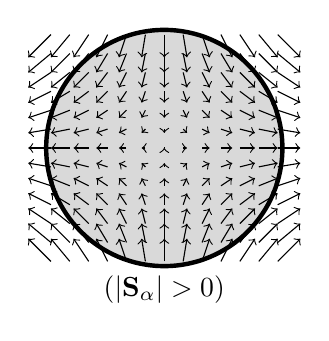
\begin{tikzpicture}[ultra thick,scale=0.6]
        \def\nRows{6}
        \def\nCols{6}
        \draw[fill=gray!30] (0,0)circle(2.5);
        \foreach \x in {-\nRows,...,\nRows} {
            \foreach \y in {-\nCols,...,\nCols} {
                \pgfmathsetmacro\distance{veclen(\x*0.4, \y*0.4)};
                \pgfmathparse{\distance < 2.5 ? "blue" : "white"}
                \edef\colour{\pgfmathresult};
                \ifthenelse{\equal{\colour}{blue}}{                    
                    \draw[thin,->](\x*0.4,\y*0.4)--++(0.08*\x,-0.08*\y);
                }
            }
        }
        \node (txt) at (0,-3){($|\textbf{S}_\alpha| > 0$)};
    \end{tikzpicture}
     \hfill
    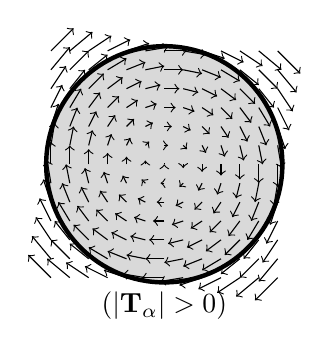
\begin{tikzpicture}[ultra thick,scale=0.6]
        \def\nRows{6}
        \def\nCols{6}
        \draw[fill=gray!30] (0,0)circle(2.5);
        \foreach \x in {-\nRows,...,\nRows} {
            \foreach \y in {-\nCols,...,\nCols} {
                \pgfmathsetmacro\distance{veclen(\x*0.4, \y*0.4)};
                \pgfmathparse{\distance < 2.5 ? "blue" : "white"}
                \edef\colour{\pgfmathresult};
                \ifthenelse{\equal{\colour}{blue}}{                    
                    \draw[thin,->](\x*0.4,\y*0.4)--++(0.08*\y,-0.08*\x);
                }
            }
        }
        \node (txt) at (0,-3){($|\textbf{T}_\alpha| > 0$)};
    \end{tikzpicture}
    \hfill
    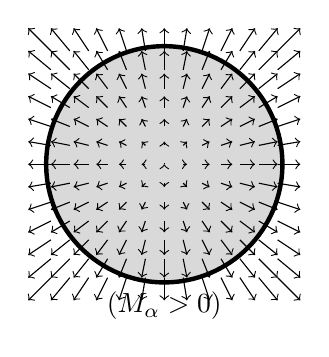
\begin{tikzpicture}[ultra thick,scale=0.6]
        \def\nRows{6}
        \def\nCols{6}
        \draw[fill=gray!30] (0,0)circle(2.5);
        \foreach \x in {-\nRows,...,\nRows} {
            \foreach \y in {-\nCols,...,\nCols} {
                \pgfmathsetmacro\distance{veclen(\x*0.4, \y*0.4)};
                \pgfmathparse{\distance < 2.5 ? "blue" : "white"}
                \edef\colour{\pgfmathresult};
                \ifthenelse{\equal{\colour}{blue}}{                    
                    \draw[thin,->](\x*0.4,\y*0.4)--++(0.08*\x,0.08*\y);
                }
            }
        }
        \node (txt) at (0,-3){($M_\alpha > 0$)};
    \end{tikzpicture}
    \hfill
    \caption{Typical values of moment of momentum. 
    The arrows represent the velocity field inside the droplets ($\textbf{w}_2^0$) with the corresponding value of the moment of momentum tensor.}
    \label{eq:scheme}
\end{figure}

Injecting, $f_2 = \rho_2$ in the second-order moment equation (derived in \ref{ap:Moments_equations}) we obtain :
\begin{equation}
    \ddt {\textbf{M}_\alpha}=2\textbf{S}_\alpha. 
    \label{eq:dt_M_alpha}
\end{equation}
which is the general form of the second moment of mass conservation equation. 
From \ref{eq:dt_M_alpha} we deduce that the evolution of the distribution of mass of a particle is solely motivated by the stretching of momentum, denoted by $\textbf{S}_\alpha$. 
This implies that the angular momentum (not to be confused with the angular velocity) plays no-role in the evolution of the second moment of the mass distribution. 
This is due to the symmetry of the tensor $\textbf{M}_\alpha$ that must be preserved after derivation. 
Note that if the particle has a constant $\textbf{M}_\alpha$ under change of reference frame, such as for spherical particles where we can write $\textbf{M}_\alpha= \frac{a^2 m_\alpha}{5} \bm\delta$, then the stretching of momentum is null $\textbf{S}_\alpha=0$ since $\ddt \textbf{M}_\alpha = 0$ in this situation.
This argument has no restriction on the internal particle motion, thus it is also true for fluides particles with possible inner motion. 
Additionally, applying the trace operator on both sides of \ref{eq:dt_M_alpha}, yields the interesting relation : $\ddt {M_\alpha}=\frac{2}{3}\bm\delta : \textbf{S}_\alpha$.
We can state that $M_\alpha = \lambda^\alpha_1(t)+\lambda^\alpha_2(t)+\lambda^\alpha_3(t)$, with $\lambda_i^\alpha$ for $i=1,2,3$, being the eigenvalues of $\textbf{M}_\alpha$.
For unreformable particles it is evident that the eigenvalues are not function of time, implying $\ddt M_\alpha = 0$.  
Consequently, $\bm\delta : \textbf{S}_\alpha$ has the notable property of being null whenever the particle shape remains constant, irrespective of the orientation.
The third invariant of $\textbf{M}_\alpha$ is related to the volume of the particle. 

Now, that we described the kinematic of the particle shape let us derive an equation for the moment of momentum. 
This equation is derived injecting $\textbf{Q}_\alpha = \textbf{P}_\alpha$ in \ref{eq:dt_Q_alpha_tot}, it reads, 
\begin{equation}
    \ddt {\textbf{P}_\alpha}
    - \intO{ \rho_2  \textbf{w}_2^0 \textbf{w}_2^0 }
    = 
    - \intO{\bm{\sigma}_2^0}
    - \intS{ 
        \gamma (\bm\delta - \textbf{nn})
    }
    + \intS{ \textbf{r}\bm{\sigma}_1^0\cdot \textbf{n}_2} 
    \label{eq:dt_P_alpha}
\end{equation}
On the left-hands side of \ref{eq:dt_P_alpha} we have gathered the inertial terms, i.e. the derivative of $\textbf{P}_\alpha$ and the internal velocity term $\intO{\rho_2\textbf{w}_2^0\textbf{w}_2^0 }$; 
The inertia of the particle is balanced by the right-hand side terms, namely : 
the integral of the particle internal stress $\intO{ \bm{\sigma}_2^0}$; 
the integral of the surface tension stress $\intS{ \gamma (\bm\delta- \textbf{nn}) }$; 
and the first moment of the hydrodynamic stress tensor, $\intS{\textbf{r}\bm\sigma_1^0\cdot \textbf{n}}$.
The last term on the right-hands side of \ref{eq:dt_P_alpha} represents the first hydrodynamic moment of the force traction on the particle surface.
One might immediately recognize that this equation is in facts an extension to Batchelor’s famous result, 
\begin{equation}
    \intO{\bm{\sigma}_2^0}
    + \intS{\gamma(\bm\delta - \textbf{nn})},
    = \intS{\textbf{r}\bm\sigma_1^0\cdot \textbf{n}},
    \label{eq:Batchelor}
\end{equation}
but with the consideration of inertia of the particle.
\ref{eq:Batchelor} is particularly useful to express the unknown internal stress within solid particles in terms of surface integral, i.e. the stress let $\intS{(\textbf{r}\bm\sigma_2^0+ \bm\sigma_2^0\textbf{r})\cdot \textbf{n}}$ and the surface tension forces.
This relation is the main tools used to express the bulk stress of a suspension, it eventually leads to the computation of the famous Einstein equivalent viscosity upon having the right closure for $\intS{(\textbf{r}\bm\sigma_2^0+ \bm\sigma_2^0\textbf{r})\cdot \textbf{n}}$. 
Therefore, the significant aspect of \ref{eq:dt_P_alpha} is that it can be interpreted as a generalized equation for the integrated stress tensor within the volume of the particle upon the knowledge of the inertial terms.
This will become particularly relevant when determining form of the total stress of an inertial suspension as it will be mentioned in \ref{sec:averaged_eq}.

The conservation equation of the angular momentum $\bm{\mu}_\alpha$ is obtained by taking the double contracted product of \ref{eq:dt_P_alpha} with $\bm\epsilon$, which gives the simple expression :
\begin{equation}
    \ddt\bm{\mu}_\alpha
    =  
    % \textbf{t}_\alpha.
    \intS{ \textbf{r} \times \bm{\sigma}_1^0\cdot \textbf{n}_2 }
    \label{eq:dt_mu_alpha}
\end{equation}
Notice that every terms on the RHS of \ref{eq:dt_P_alpha} vanish due to their symmetric nature apart from the shew-symmetric part of the hydrodynamic stress, which is the hydrodynamic torque applied on the particle $\alpha$.
Particularly, the surface tension terms do not appear in the angular momentum balance since $\bm\sigma_I^0 = \gamma (\bm\delta-\textbf{nn})$ is symmetric, which is consistent with the findings of \citet{hesla1993note}. 
As a consequence, the surface tension has no effect on the angular momentum regardless of the particle's shape. 
In the literature it is common to include the torque due to inter-particular interactions in the angular momentum balance, as it is done in \citet{jackson1997locally} and \citet{zhang1997momentum}.
In our case note that $\bm{\sigma}_0^1$ contains also the short range interaction forces.

Taking the double contracted product of \ref{eq:dt_Q_alpha_tot} with the tensor $\frac{1}{3}\bm\delta$, directly yields the scalar equation for the 
\begin{equation}
    \frac{1}{2}\ddt^2 {M_\alpha}
    - \frac{1}{3}\intO{ \rho_2 \textbf{w}_2^0 \cdot \textbf{w}_2^0}
    = 
    \intO{p_2^0} 
    % - \frac{1}{3}\intS{p_1^0 \textbf{r}\cdot \textbf{n}}
    - \frac{2}{3} \gamma s_\alpha
    - \frac{1}{3}\intS{p_1^0 \textbf{r}\cdot \textbf{n}}
    + \frac{1}{3}\intS{\textbf{r}\cdot\bm\tau_1^0\cdot \textbf{n}}
    \label{eq:dt_D_alpha}
\end{equation}
where we have made use of the explicit form of the Newtonian stresses $\bm\sigma_k^0 = p_k^0 \bm\delta + \bm\tau_k^0$, to highlight the role of the pressure. 
This, corresponds to the isotropic work balance within the particle's volume and surface. 
As a matter of fact, the rate of compression of a particle, denoted by the second derivative of $M_\alpha$ evolves according to : 
the internal kinetic energy, $\intO{\rho_2 \textbf{w}_2^0 \cdot \textbf{w}_2^0 }$;
the particle internal pressure, $\intO{ p_2^0}$; 
the surface energy $\intS{ \gamma }$; 
and the trace of the hydrodynamic first moment.
If one consider spherical particles \ref{eq:dt_D_alpha} corresponds to the Rayleigh-Lamb equation.  
Additionally, in the steady-state case one recover from \ref{eq:dt_D_alpha} Young–Laplace equation. 



Taking the symmetric and traceless part of \ref{eq:dt_P_alpha}, and by making use of \ref{eq:dt_M_alpha} yield a dynamical balance equation for the traceless part of $\textbf{M}_\alpha^\text{dev}$, namely
\begin{multline}    
    \frac{1}{2}\ddt^2{\textbf{M}_\alpha^\text{dev}}
    - \intO{\left(
        \rho_2\textbf{w}_2^0 \textbf{w}_2^0
        - \rho_2\frac{1}{3}(\textbf{w}_2^0 \cdot \textbf{w}_2^0)\bm\delta\right)}
    =  
        - \mu_2 \intO{\textbf{e}_2^0}
        - \intS{\gamma\left(\frac{1}{3}\bm\delta-\textbf{nn}\right)}\\
        + \frac{1}{2}\intS{\left(\textbf{r}\bm\sigma_1^0+ \bm\sigma_1^0\textbf{r} - \frac{2}{3}(\bm\sigma_1^0\cdot \textbf{r})\bm\delta\right)\cdot \textbf{n}}
    \label{eq:dt_S_alpha}
\end{multline}
where $\textbf{M}^\text{dev}_\alpha = \textbf{M}_\alpha - M_\alpha$ is a measure of the particle aspect ratio since for spherical particles $\textbf{M}^\text{dev}_\alpha = 0$.
On the left-hand side of \ref{eq:dt_S_alpha} we recover the deviatoric part of the inertial contributions. 
On the right hand-side we can identify the terms responsible only for the droplet deformation, excluding expansion and compression effects.
Notice that the internal particle pressure does not play a role in this equation.  
The surface tension tensor $\intS{\gamma\left(\frac{1}{3}\bm\delta-\textbf{nn}\right)}$ is therefore the deviatoric tensor responsible only for the deformation. 
An finnaly the external contribution $\frac{1}{2}\intS{\left(\textbf{r}\bm\sigma_1^0+ \bm\sigma_1^0\textbf{r} - \frac{2}{3}(\bm\sigma_1^0\cdot \textbf{r})\bm\delta\right)\cdot \textbf{n}}$ is a quantity close to what we call the stresslet. 

It is now clear that if the surface tension forces play no role in the linear and angular momentum equation, it does impact the moment of momentum $\textbf{P}_\alpha$ or more specifically its symmetric part $\textbf{S}_\alpha$.
Thus, the surface tension force impact the hydrodynamic behavior of a particle solely through its action on $\textbf{S}_\alpha$, which is related to the shape of a particle through \ref{eq:dt_M_alpha}.
As remarked by \citet{batchelor1970stress}, since the surface tension force oppose the deformation of a particle, it can be understood as an elastic force. 
Which, as it will be shown in \ref{sec:averaged_eq} has a role on the bulk stress of the suspension. 
% Additionally, note that \ref{eq:dt_S_alpha} can be seen as a formula to reformulate the integral of the internal stress $\pOavg{\bm{\sigma}}$.
Additionally, in \ref{ap:Moments_equations} we show how to derive the higher order moment of momentum equations, which can also be viewed as formulas for the higher moments of the internal particle stress distribution. 
It is interesting to mention that in a recent study of \citet{dolata2021faxen} and \citet{zhou} they use energy method and recover the first two moments of momentum equations hidden into another but equivalent form, valid in the stokes flow regime. 



